\section{Data and Methodology}
As the largest electronic retailer in the U.S, Amazon was reported to have 270 active customer accounts in 2014 \footnote{http://www.statista.com/statistics/237810/number-of-active-amazon-customer-accounts-worldwide}. With such large user base, user behavior in Amazon significantly imply the market pattern and preference, which is critical for electronic commercials and advertisement ecosystem. However, such online user behavior has not been systematically studied before. In this paper we unveil customer shopping pattern in Amazon through analyzing Wishlists of a large amount of users.

Every registered user in Amazon has a public profile that contains various objects such as profile photo, rated items, reviews, and Wishlists, etc. Wishlist is a list-type object that contains the desired products added by the user. A user may have multiple Wishlists to accommodate different types of products. Wishlists can be useful in many ways. For examples, a user may use Wishlists to record the products he/she wishes to buy in the future. Or the user may use the Wishlist to show guidelines for gift givers. Beside items, each wishlist maintains a separate recipient profile, including name, birthday, and shipping address. When a new Wishlist for the user is created, birthday and address are defaulted to be empty, and recipient name is pre-set as the user's profile name. To preserve user privacy, birthday has only month and day in a Wishlist, thus the age of the recipient is unknown. Similarly, address information shows only the state and city. Note that although every user has a public profile, not all objects in this profile are public. Wishlists are configurable yet public in default. We focus on the analysis of user Wishlists. Therefore, other objects that are beyond the scope of this paper such as reviews, activities are deliberately omitted.

Figure~\ref{data_struct} shows the data hierarchy in our measurement. We illustrate only the layers under the Wishlist. As we can see from the figure, other than items, each list has its own recipient name, birthday, and address. Beside these formated information, each Wishlist can have a list-description. List-description is plain text keyed in by the users, which is which is usually used to briefly introduce the wishlists and the users. Examples are \emph{``I LOVE music! Buy me a CD!"} or \emph{``Son of Sue and Kevin, brother of Roger, husband of Kathy. I moved from Milton Keynes, England to Smithfield, North Carolina, USA on 8/8/2000 and recently moved from there to the Raleigh/Garner border in the same state"}. The first example list-description shows the hobby of a user and the second example exposes much more personal information such as parents' names, marriage status, wife name, moving history, etc. 

\begin{figure}[h!].
\centering
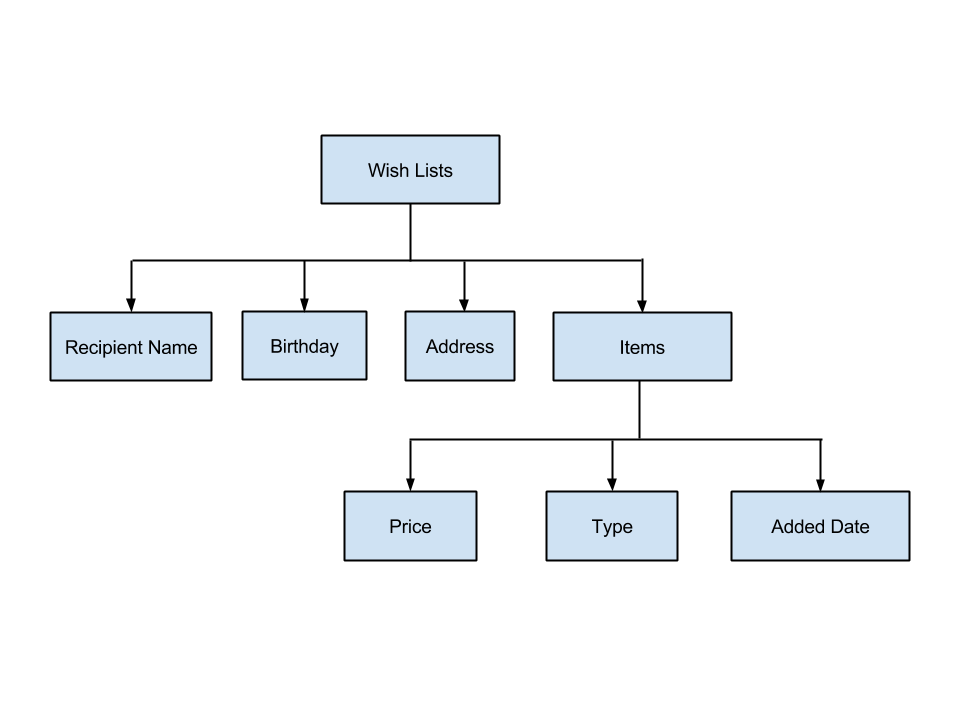
\includegraphics[width=.45\textwidth]{data_struct.png}
\caption{data hierarchy}.
\label{data_struct}
\end{figure}

As the Wishlist stores the user desired products, it directly reflect the user online shopping pattern in Amazon. Particularly we are interested in the products users prefer to buy, the time when shopping peak or pit happens, and the price users are willing to pay. Therefore we need to collect adequate number of data from Amazon for analysis. 

\subsection{Data Collection Methodology}
One way to collect data from Amazon is to use its Product Advertising API[]. However, the API does not provide wishlist or product type accesses, which are essential in our study. Besides, there is a 1 request/second limit on non-profiting API users (The actual rate is $1 + round({S\over \$4600})$[], in which $S$ denotes the sales in the user's website in last 30 days). Using few API accounts does not boost the speed while signing up for more accounts require much more effort. Therefore we opt for crawling Amazon by web scraping. Although web scraping may not be reliable, it provides all information that are needed. We implement the crawler using python package BeautifulSoup [] to extract specific data in certain HTML tags. 

Generally the data collection process consists of 3 steps. In each step we store certain data and collect input data for the next step. 

First we aim to collect substantial amount of user profiles to expand our crawling targets. From the user profile, we are able to extract the user name, birthday, address, Wishlist names, list URLs, and Wishlist list-descriptions. To this end, we leverage Amazon wishlist search engine~\footnote{http://www.amazon.com/gp/registry/search} to search common names. The wishlist search engine will return at most 2016 users and that are associated with a name. \footnote {The search engine usually states that hundreds of thousand users are found, but only the first 2016 users are viewable.} We have mentioned that each Wishlist under a user profile may have different personal information such as name, address, etc. The search engine returns the user name, birthday, address, and list-description as the ones in the latest updated Wishlist. Figure~\ref{searcheng} shows the result of a typical search, in which we searched user named ``Paul".


\begin{figure*}[!htb]
\minipage{0.32\textwidth}
  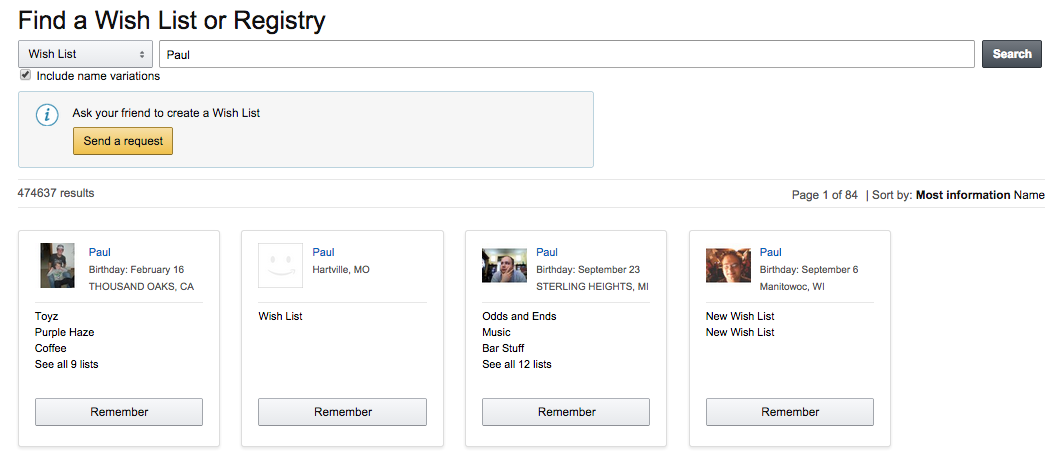
\includegraphics[width=\linewidth]{searcheng.png}
  \caption{Wishlist Search Engine}\label{searcheng}
\endminipage\hfill
\minipage{0.32\textwidth}
  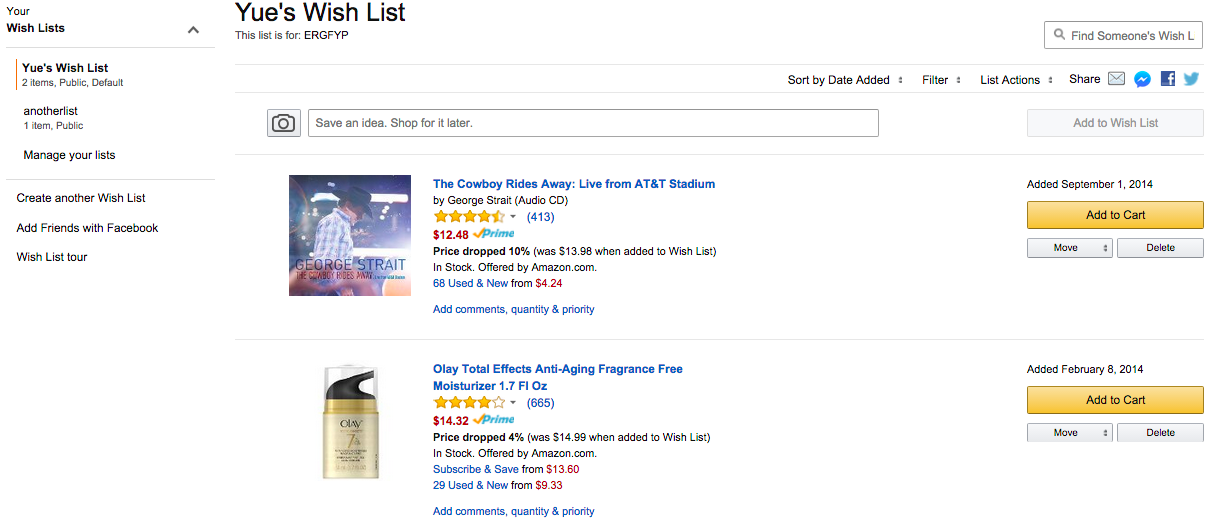
\includegraphics[width=\linewidth]{listitem.png}
  \caption{Wishlist}\label{listitem}
\endminipage\hfill
\minipage{0.32\textwidth}%
  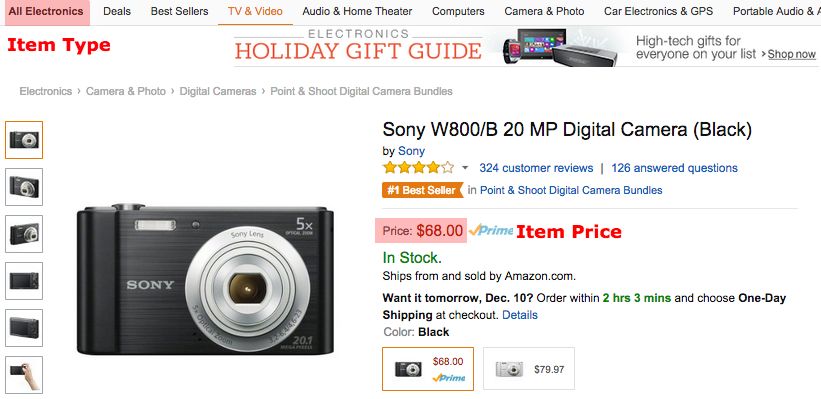
\includegraphics[width=\linewidth]{item.png}
  \caption{Item}\label{item}
\endminipage
\end{figure*}

Then we further investigate the items in the Wishlist. We directly visit the Wishlist URLs extracted in last step. In the page of Wishlist as shown in Figure~\ref{listitem}, the items are listed with links to their own pages. We cannot know the price and type of the item until we visit these pages. Therefore to this point we are only able to collect item name, item page URL and the date the items were added. 

Finally We retrieve detailed information for each item. We visit all the item URLs and download the product pages. One example of the product web pages is shown in Figure~\ref{itempage}. In a page like this, the item type and the item price (In red box) can be easily extracted. However, there may not always be only one price for an item. For example, for the same item, there can be prices from different retailers. There are also differences between new ones and used ones. We record only the price that the wishlist owner chose (Wishlists remember which version of the items are selected in most cases). In cases which the user does not choose a price, we record the lowest prices that a user needs to pay to get an item. In these rare case we believe it is reasonable to choose the lowest price because it is natural to assume that people prefer to pay less to purchase an item. Note that we cannot always find the price for an item. There are multiple reasons -- (1) The item is removed from Amazon so there is no web page for it. However, it still stays in user Wishlists. (2) The item is no longer in stock, the price shown will be ``Currently unavailable" (3) Web failures and anti-crawler mechanisms.

\subsection{Data Overview}
We searched the top 300 common male and female names \footnote{http://names.mongabay.com/} to harvest user profiles. Eventually we collected 1,233,095 unique users.Their profile information and wishlist links are stored in our database. However, collecting Wishlists of all the users is very time-consuming (Consider that one Amazon product Page usually has over 10 thousand lines of code, which is around 300KB data). Therefore we collect only part of the user profile pool that is large enough to conduct sound measurement. As we are also interested in personal information of a user, we collect the wishlists and items of users who potentially have input personal information -- users with list-description. To this end, we collected 30,057 complete user, together with all the items and wishlists. In total we collected 76,923 wishlists and 5,710,674 items, among which 2,248,142 are unique. The size of the data is approximately 1.6GB. 


\subsection{Personal Information}
Although we did not collect wishlists for all the recorded users. We can still use their wishlist profile to study personal information exposure in Amazon especially when we are particularly interested in potential user information leakage. Table~\ref{tb:stat} illustrates information exposure in user list profiles. We found that a considerable number of users put their birthday and location information in their list profiles. Furthermore, most of the people who have a list-description have exposed their birthday and address information. Our findings agree with \cite{frankowski2006you}, which states that users tend to expose their personal information in open websites. 

\begin{table}[!htbp]
\centering
\caption{Personal Information in User Profile}
\label{tb:stat}
\begin{adjustbox}{max width=.5\textwidth}
\begin{tabular}{lll}
Personal Info & User Number & Percentage \\
Birthday & 280,328 & 29.0\% \\
Location & 221,298 & 22.9\% \\
Birthday \& Location & 150,004 & 15.5\% \\
List-description & 104,846 & 10.8\% \\
List-description \& Birthday & 94,284 & 9.7\% \\
List-description \& Location & 59,731 & 6.2\% 
\end{tabular}
\end{adjustbox}
\end{table}

